\section{Efficiency Focused Platforms} \label{chapter3:software-efficiency}

To cope with the limitations the previous section concludes on, both the academia and the industry suggested solutions discarding productivity to focus on efficiency.
Among these solutions, the concurrent and parallel programming paradigms are presented in section \ref{chapter3:software-efficiency:concurrency}
They are evaluated against the same criteria than the previous section - Productivity, Efficiency and Adoption.
This evaluation illustrates the impact of this shift of focus on the adoption of these platforms, as presented in section \ref{chapter3:software-efficiency:adoption}.
Finally, section \ref{chapter3:software-efficiency:productivity-limitations} presents the limitations of parallelism on productivity.

\subsection{Concurrency} \label{chapter3:software-efficiency:concurrency}

\begin{figure*}[h!]
\textfig{%
  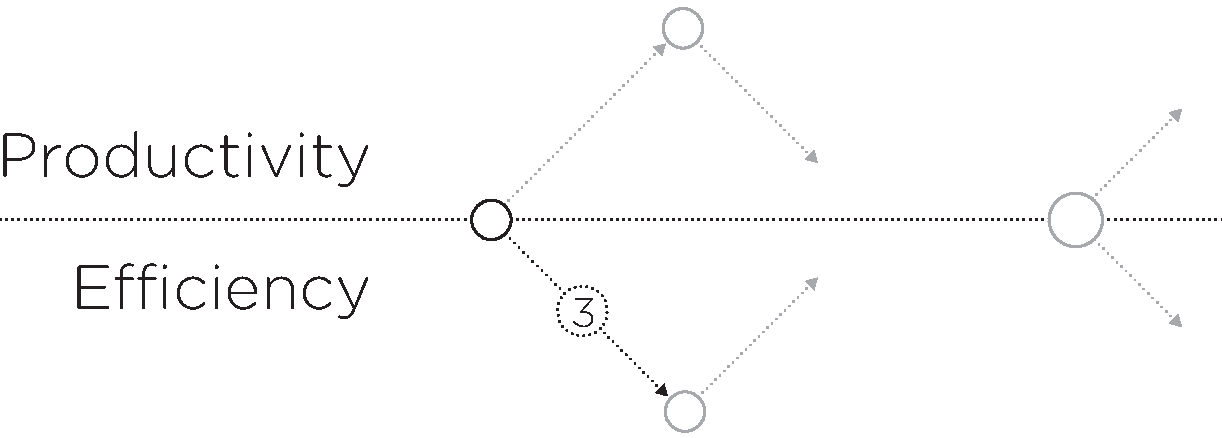
\includegraphics[width=0.6\textwidth]{../resources/state-of-the-art-3.pdf}%
  % \caption{Focus on Efficiency}%
  % \label{fig:state-of-the-art-3}%
}%
\end{figure*}

Web servers need to be able to process lots of concurrent operations in a scalable fashion.
Concurrency is the ability to make progress on several operations roughly simultaneously.
It implies to draw memory boundaries to define independent regions, or to define causality in the execution of tasks.
When both boundaries and causality are clearly defined, the tasks are independent and can be scheduled in parallel to make progress strictly simultaneously.

The definition of independent tasks allows the fine level synchronization within a task, and coarse level message passing between the tasks required for performance efficiency.
The synchronization of execution at a fine level assures the invariance on the shared state, and avoid communication overhead.
The message-passing at a coarser level assures the parallelism.
The two are indispensable for efficiency.

\subsubsection{Concurrent Programming} \label{chapter3:software-efficiency:concurrency:concurrent-programming}

% \cit{Building concurrent programming is like building a steam engine through a keyhole}{TODO}

\cit{No matter how great the talent or efforts, some things just take time. You can't produce a baby in one month by getting nine women pregnant.}
{Warren Buffett\ftnt{http://bit.ly/warren-buffet-quote}}

% \illustration{TODO feu rouge et rond point}
Concurrent programming provides the mechanisms to assure atomicity of concurrent operations.
They define the causal scheduling of execution and assure the invariance of the global memory.
There are two scheduling strategies to execute concurrent tasks on a single processing unit, cooperative scheduling and preemptive scheduling.

\begin{description}
\item[Cooperative Scheduling] allows a concurrent execution to run until it yields back to the scheduler.
Each concurrent execution has an atomic, exclusive access on the memory.
\item[Preemptive Scheduling] allows a limited time of execution for each concurrent execution, before preempting it.
It assures fairness between the tasks, such as in a multi-tasking operating system.
But the unexpected preemption breaks atomicity, the developer needs to lock the shared state to assure atomicity and exclusivity.
\end{description}

The event-driven programing model relies on cooperative scheduling, and the multi-threading programming model relies on preemptive scheduling.
% Additionally, they present two alternatives to these two main programming models, lock-free data-structures and Hybrid models.

\paragraph{Event-Driven Programming}

In the event-driven execution model, developers explicitely split the application into several concurrent tasks called handlers.
The execution model schedules these handlers sequentially with the queue of events, to assure exclusivity on shared resources, and cooperatively to assure atomicity.
Moreover, they communicate with the resources asynchronously to avoid waiting.
A handler yields execution to the next handler to complete the communication.

Promises were introduced as an help to nicely chain these concurrent handlers \cite{Liskov1988}.
A promise is a placeholder for a future result allowing to defer operations for when the result is available.
It layouts the concurrent handlers in chains, similarly to a pipeline.

This execution model is very efficient for highly concurrent applications as it avoids contention.
Several platform rely on this execution model, like \ImplementationsOf{Event-driven programming}.
As well as some web servers like Flash \cite{Pai1999}, Ninja \cite{Gribble2001} thttpd\ftnt{http://acme.com/software/thttpd/} and Nginx\ftnt{https://www.nginx.com/}.

Though, the event-driven model is limited in performance because of the global memory.
The handlers cannot be scheduled in parallel.
Lock-free data-strincture intends to improve performance by reducing the atomic portions of operations to a minimum.

\paragraph{Lock-Free Data-Structures}

The wait-free and lock-free data-structures use atomic operations small enough so that locking is unnecessary \cite{Lamport1977,Herlihy1988,Herlihy1990,Herlihy1991,Anderson1990}.
They provide concurrent implementations of basic data-structures such as \ImplementationsOf{Lock-free Data-Structures}.
They rely on instructions provided by transactional memories \cite{Harris2010} that combine read and write instructions.

Lock-free Data-structures allow parallelization of the concurrent tasks, but are mostly unavailable on common hardware.
Multi-threading intends to provide parallelization with software protection.

\paragraph{Multi-Threading Programming}

Threads are small execution containers sharing the same memory execution context within an isolated process \cite{Dijkstra1968}, and scheduled in parallel with fork/join instructions \cite{Randall1998,Frigo1998,Leiserson2010}.
They execute statements synchronously and are preempted to avoid blocking the progression of other threads.
Without protection, the preemption breaks the atomicity and exclusivity of memory accesses.
To assure atomicity and exclusivity, hence invariance, multi-threading programming models provide protection mechanisms, such as \ImplementationsOf{Multi-threading programming}.

Developers tend to use the global memory extensively, and threads require to protect each and every shared memory cell.
This heavy need for synchronization leads to bad performances, and is difficult to develop with \cite{Adya2002}.

\paragraph{Hybrid Models}

Hybrid models intend to join the productivity advantage of synchronous execution from thread, with the efficiency advantage of asynchronous execution from events-driven models.
The implementations of hybrid models are \ImplementationsOf{Hybrid Models}.
For example, cooperative threads, or fibers, avoid splitting the execution into atomic tasks nor use protection mechanisms to assure exclusivity.
A fiber yields the execution to another fiber to avoid blocking the execution during a long-waiting operation, and recovers it at the same point when the operation finishes.
However, it wasn't adopted in practice.
Hiding the yielding points effectively hide the preemption.
Developers cannot protect atomicity of operations, which increases the likeliness of race conditions \ftnt{http://bit.ly/deciphering-glyph-unyielding}.

\paragraph{Limitation of Concurrent Programming}

The presented concurrent programming paradigms assure sequentiality of execution within a task and the causal ordering between tasks.
Multi-threading imposes heavy protection mechanisms and fails to avoid contention because of the preemptive scheduling.
Hybrid models try to improve over multi-threading using cooperative scheduling.
But the synchronous execution imposed by these two models is excessive.
It impacts performance, and is difficult to manage efficiently.

The causal ordering between tasks proposed by the event-driven execution model is sufficient to assure correctness of execution \cite{Lamport1978,Reed2012}.
And it is easier for developer to define causal scheduling than to assure the consistency of memory with protection mechanisms.
But because of the lack of memory isolation, the concurrent tasks are not scheduled in parallel.
It impacts efficiency, as detailed in table \ref{tab:efficiency-parallel}.
Parallel programming is the only solution for efficiency, at the expense of development efforts to explicitly define the memory isolation of concurrent tasks and their communications by message passing.

\subsubsection{Parallel Programming} \label{chapter3:software-efficiency:concurrency:parallel-programming}

The Flynn's taxonomy \cite{Flynn1972} categorizes parallel executions in function of the multiplicity of their flow of instruction and data.
Parallel programming models belong to the category Multiple Instruction Multiple Data (MIMD), which is further divided into Single Program Multiple Data (SPMD) \cite{Auguin1983,Darema1988,Darema2001} and Multiple Program Multiple Data (MPMD) \cite{Chang1997,Chan2004}.
SPMD defines a single program replicated on many processing units \cite{Culler,Johnson1995,K.ManiChandy2005} -- it is roughly derived from the multi-threading programming model presented above.
While MPMD defines multiple parallel tasks in the implementation \cite{Grimshaw1991,Foster1995b,Foster1996}.
The two major theoretical models for MPMD parallel programming are the Actor Model and Communicating Sequential Processes.

% \nt{schema of SPMD and MPMD}

\paragraph{Actor Model}

The Actor Model allows to express the causal ordering of computation as a set of parallel actors communicating by asynchronous messages \cite{Hewitt1973a, Hewitt1977, Clinger1981}.
In reaction to a received message, an actor can create other actors, send messages, and choose how to respond to the next message.
In reality, communications are too slow compared to execution to be synchronous, and are subject to various faults and attacks \cite{Lamport1982}.
The Actor model takes these physical limitations into account \cite{Hewitt1977a}.
\paragraph{Communicating Sequential Processes}

Similar works include the Communicating Sequential Processes (CSP) \cite{Hoare1978, Brookes1984}, and the Kahn Networks \cite{Kahn1974, Kahn1976}.
Coroutines are autonomous programs which communicate with adjacent modules as if they were input and output subroutines \cite{Conway1963}.
It defines a pipeline to implement multi-pass algorithms.

The difference between Actors and Coroutines lie in the definition of the communication.
Actors send messages to named actors, whereas Coroutines communicate through named channels.

\subsubsection{Summary of Concurrent and Parallel Programming Models}

Compared to parallel programming, the concurrent programming models are unable to correctly isolate the concurrent tasks and communicate by message-passing to allow parallelism.
Hence the parallel programming models are more efficient than the concurrent programming models, as detailed in table \ref{tab:efficiency-parallel}.

\ParallelEfficiencyTable{tab:efficiency-parallel}

\subsection{Steering Back Toward Producitivity} \label{chapter3:software-efficiency:adoption}

\begin{figure*}[h!]
\textfig{%
  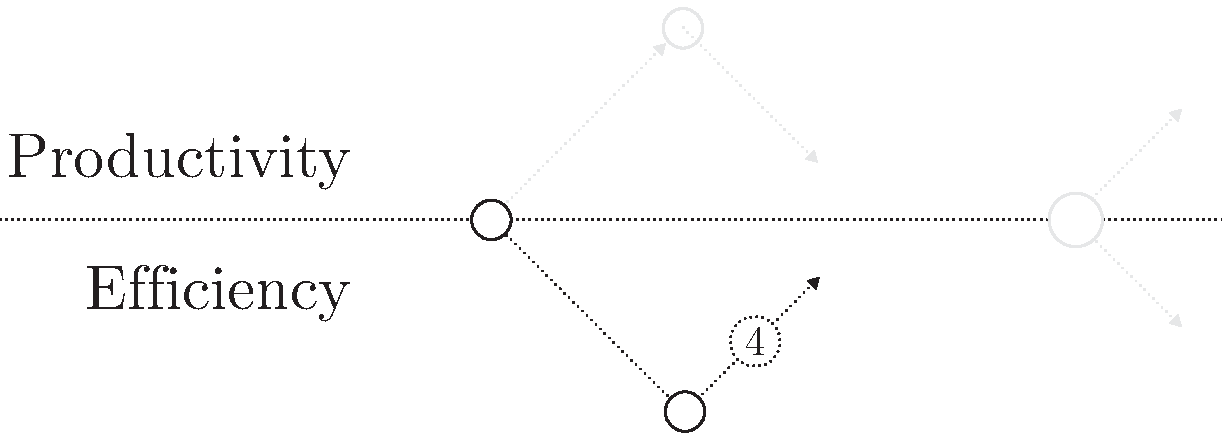
\includegraphics[width=0.6\textwidth]{../resources/state-of-the-art-4.pdf}%
  % \caption{Steering back toward Productivity}%
  % \label{fig:state-of-the-art-4}%
}%
\end{figure*}

When the need for efficiency is higher than the need for productivity, the adoption is steered by the industry more than the community.
If the industry really needs a platform, it will commit the required development effort despite low productivity.

\marginfig{10}{0.6\textwidth}{
  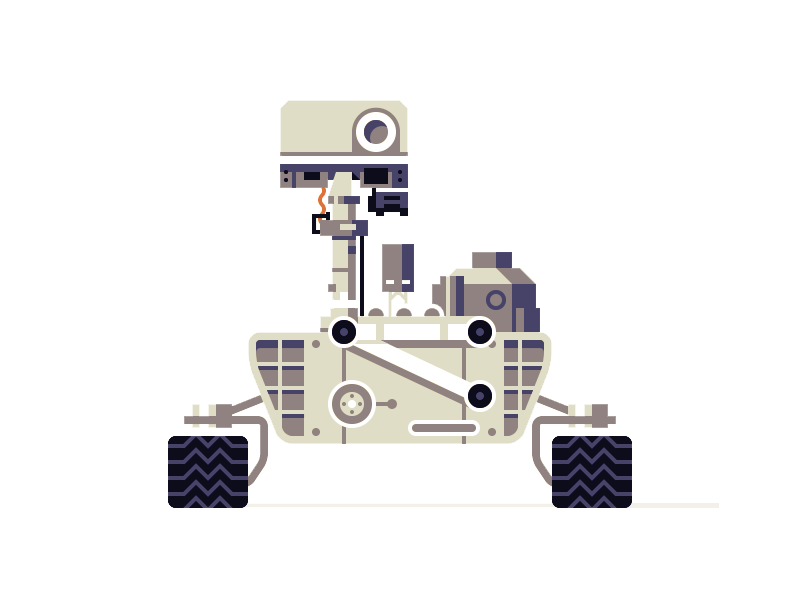
\includegraphics[width=0.4\textwidth]{../resources/marsrover.png}
  \illustration{Justin Mezzell \url{http://bit.ly/justin-mezzell-curiosity}}
}

The platforms for the Mars Rovers or some banking systems are about 30 years old, yet the industry continues to maintain them.
The platform presented in this section emerged from the academia and the industry but are often barely known by the larger community of developers.
The more the platform trades productivity for efficiency, the less support it receives from the community.


\subsubsection{Concurrent Programming}

Most programming language implementations support concurrent programming.
Either with multi-threading or event-driven programming.
These two are highly adopted by both the industry and the community, as presented in table \ref{tab:efficiency-adoption}.

On the other hand, lock-free data structures and cooperative threads comes from the academia, similarly to functionnal programming, and did not encounter significant adoption from the community.

\subsubsection{Parallel Programming}

Several platforms were directly inspired by the actors model, like \ImplementationsOf{Actor Model}.
Scala is a programming language unifying the object model and functional programming.
Akka is a framework based on Scala, following the actor model to build highly scalable and resilient applications.
Play is a web framework based on top of Akka.
And Erlang is a functional language designed by Ericsson to operate networks of telecommunication devices \cite{Armstrong1993,Nelson2004,Armstrong2014}

Other platforms were inspired by other theoretical model, like \ImplementationsOf{Communicating Sequential Processes}, inspired by Coroutines and CSP.
Go is an open source language initiated by Google to build highly concurrent services.

These examples of implementation are largely used in the industry, but are almost unknown outside of it.
They are backed by strongly passionated but small communities.

Indeed, it is difficult for developers to manage the superposition of these two organizations, tasks and modules.
The organization in independent tasks is hardly compatible with the modular organization presented in the previous section.
This superposition makes these platforms accessible only to an elite in the industry supporting it.
To mitigate this difficulty, various platforms help organizing the tasks, or adopt the same granularity for modules and tasks to fit the two organizations.

\paragraph{Tasks Organization and Communications}

To reduce the difficulties of the superposition of tasks and modules, algorithmic skeletons propose predefined patterns of organization to fit certain types of problems \cite{Cole1988, Dean2008, McCool2010, Gonzalez-Velez2010}.
Developers focus on their problem and delegate the communications to specialized skeletons.
These solutions are hardly used by the community, but are crucial in some industrial contexts.
A famous example is the map/reduce pattern introduced by Google \cite{Dean2008}.

\paragraph{Tasks Granularity}

The Service Oriented Architectures (SOA) allows developers to express an application as an assembly of services connected to each others.
Some examples of SOA platforms are \ImplementationsOf{Service Oriented Architecture}.
It allows to adjust the granularity of tasks to help developers to better fit the tasks organization with the modular organization \cite{Adam2008}.

More recently, Microservices are tackling the same challenge on the web, with a finer granularity \cite{Fernandez-Villamor2010,Fowler2014,Namiot2014}.
An example of Microservice platform is \ImplementationsOf{Microservices}.
Microservices are very recent, and it is difficult to asses their usage in the community nor the industry.
But they seem to be increasingly adopted, both in the industry and in the community.

\separator

The parallel programming platforms previously presented allow to build generic distributed systems.
In the context of the web, a real-time application must process high volumes streams of requests within a certain time.
This requirement imposes specific challenges for the platforms.

\subsubsection{Stream Processing Systems}

\paragraph{Data-stream Management Systems}

Database Management Systems (DBMS) historically processed large volumes of data, and they naturally evolved into Data-stream Management System (DSMS) to process data streams as well.
Because of this legacy, they are in rupture with MPMD platforms presented until now.
They borrow the syntax from SQL to run requests in parallel on continuous data streams.
The computation of these requests spread over a distributed architecture.
Some recent examples are \ImplementationsOf{Data Stream System Management}.

\paragraph{Pipeline Stream Processing}


On the other hand, the pipeline architecture is directly inspired by the Actors Model and CSP.
It organizes an application as a network of event-driven stages connected by explicit queues, the output of one feeding the input of the next \cite{Welsh2001}.
The event-driven paradigm of a stage is similar to work like Ninja \cite{Gribble2001} and Flash \cite{Pai1999} previously presented.
But the independence of stages allow to spread the execution on a parallel architecture.
The academic works and industrial implementations of pipeline architecture are \ImplementationsOf{Pipeline Stream Processing}.

\separator

Parallel programming emerges mainly from industrial needs and academic research but is barely supported by the community.
The implementations improve efficiency.
But their weak productivity prevents their adoption by the community.
As summarized in table \ref{tab:efficiency-adoption}, the event-driven programming model is the best candidate for a concurrent programming model regarding adoption.
It is supported by the community, and responds to concrete needs in the industry.

\ParallelAdoptionTable{tab:efficiency-adoption}

\subsection{Productivity Limitations} \label{chapter3:software-efficiency:productivity-limitations}

Parallel programming requires the organization of execution and memory into independent tasks.
This independence imposes different granularity of state accessibility.
At a fine level, the state is shared, while at a coarser level, it is isolated.
It avoids higher-order programming.
Hence, it limits the composition of modules and negatively impacts productivity.

Without this composition between modules, parallel programming forces to develop two mental representations -- one for the module organization and one for the task organization -- or to abandon the module organization and productivity altogether.
It makes parallel programming accessible only to an elite of developers that are able to be productive despite the two mental representations, as presented in table \ref{tab:efficiency-productivity}.

\EfficiencyProductivityTable{tab:efficiency-productivity}

\subsection{Summary} \label{chapter3:software-efficiency:summary}

The parallel programming platforms presented in this section focus more on efficiency than productivity.
Whereas the concurrent programming platforms feature better productivity.
But no platform features both productivity and efficiency, as presented in table \ref{tab:efficiency-synthesis}.
Moreover, this lack of versatility impacts adoption.
These platforms remain inaccessible for the community.
Exception for Event-driven and Multi-threading programming which are among the productive ways to achieve concurrency.

\EfficiencySummaryTable{tab:efficiency-synthesis}



\endinput

Streaming
\cite{Madsen2015}
\cite{Sun2015}

Map Reduce
\cite{Yao2015}


Web assembly
https://medium.com/javascript-scene/what-is-webassembly-the-dawn-of-a-new-era-61256ec5a8f6